\chapter{\label{ranking-algorithms}Ranking algorithms}

\section{What problem do a ranking algorithm solve?}

The main purpose of the algorithms discussed below in this section is to answer the question \emph{Given a score, what is the rank of a user or item with this score?} \cite{codejam}. The opposite question -- \emph{Given a rank, what is the score for this rank?} is very similar but not adressed here directly even though most approaches to the ranking problem indirectly answers that question too.

\section{\label{definition}What is ranking?}

\begin{shaded}
  
  What is ranking, formal definition
 
The rank of a well-founded set is defined inductively as the smallest ordinal number greater than the ranks of all members of the set.[1] In particular, the rank of the empty set is zero, and every ordinal has a rank equal to itself.
\href{https://en.wikipedia.org/wiki/Von\_Neumann\_universe}{Wikipedia - Von Neumann universe}

Well founded relation:

$\forall S \subseteq X ( S \neq \varnothing \rightarrow \exists m \in S \forall s \in S (s, m) \notin R)$ \href{https://en.wikipedia.org/wiki/Well-founded\_relation}{Wikipedia - Well-founded relation}

Define ordinal (each ordinal is the well-ordered set of all smaller ordinals?)

\end{shaded}

\subsection{Types of ranking algorithms}

Ranking algorithms can coarsely be divided in two categories: \emph{exact} and \emph{approximating} algorithms. The exact algorithms deal with the ranking problem by sorting and counting. The sorting part is commonly accomplished by indexing the score-property of the entity or the corresponding column in a table in case a relational database is used.  

As mentioned in the introduction, obtaining an exact rank may not be necessary. Other considerations such as speed and cost may be more important. Approximating algorithms estimate the rank by linear interpolation within a segement of ranks. Suitable segments can be found with an \emph{offline-method} such as scanning all scores periodically keeping track of scores at the segments boundaries (See section \ref{bucket}) or with an \emph{online-method} with a \emph{streaming algorithm} that maintains a model for estimating ranks by continuosly updating a number of statistical measures.

\subsubsection{Stability}
\todo{Consider removing 'Stability'}

In both cases a sorted list needs to be created. If the chosen sorting algorithm is not stable the ranking will be non-deterministic. This may or may not be a problem depending on the application. 

\todo{Strategies as in \href{https://en.wikipedia.org/wiki/Ranking\#Strategies\_for\_assigning\_rankings}{Ranking (Wikipedia)}?}

\section{Exact algorithms}

\subsection{Rank by counting}

From the \hyperref[definition]{definition of ranking} we can quite simply arrive in a solution for obtaining the rank for a score. This would be the naive solution -- getting the rank by counting the number number of highscores greater than the score in question.

This way of getting the rank can be done with a simple query in SQL
\texttt{SELECT count(id) FROM Highscores WHERE Score > TheScore} or by increasing a counter while iterating through an ordered set of highscores in case a non-relational database is used. In any case the items should be indexed on the highscore-field.

Nevertheless, obtaining rank for a score by this method implies scanning through all items having a score higher than the one you want to obtain the rank for. The time complexity of this approach is obviously $\mathcal{O}(n)$ making it unusable for online applications in terms of cost and response time\footnote{If the ranking function is not required to return a new rank, the actual rank could be assigned periodically by a background job to all the highscores. In this case the $\mathcal{O}(n)$ time complexity would be more tolerable.}.

\iffalse
\begin{shaded}

 \emph{I want to define ranking by counting like this:}

  1. define a set of items, and an item i with score s.

  2. define a sorted list of those items or someway indicate that the set is sorted by some relation

\textbf{either}
  
  3a. assign ordinal numbers to the items \\
  4a. get the ordinal number for the i.

 \textbf{or}

  3b. count items before i

\textbf{or}

  3c. Better way of counting items ``before'' the new item?
  
\end{shaded}
\fi

\subsection{Tree based approach}

As described above, ranking is fundamentally a counting problem. One way to accomplish counting more efficiently is by storing the count of each score in an N-ary tree. Each non-leaf node defines a score range and its associated count and the leaves represents individual items from the value domain, ie discreete scores.

Score updates and getting the rank for a score with this algorithm has a time complexity of $\mathcal{O}(\log{} n)$. Since fetching or updating a node may be relatively expensive in case it has to be fetched from a database system the number of ranges per node needs to be chosen so that the height of the tree remains reasonable low\footnote{The Google Code Jam Ranking Library uses 100 buckets per node}. The height of the tree is $ceil(log_{rangesize}numscores)$.

There are a number of things to consider with this approach. First, to get exact rankings the trees leaf nodes need to have as many children as there are possible scores. One way to get around that problem could be to not store individual scores but ranges. This could be done in at least two ways; by defining the ranges in beforehand or by compressing the tree at some interval so that if a childs score range has only a small frequency of its scores, then just dont build the tree further from that child. This is essentially the solution proposed by Shrivastava et al\cite{quantile_digest} with their Quantile Digest algorithm. The solution would then not be able to give exact ranks for scores.

Also, the the score distribution need to be known or the tree need to adapt to the changing score distribution over time to get an optimal solution.

\begin{figure}[h!]
  \centering
  \caption{Example of how ranking is done using a tree-based approach. To get the rank for score 30, start by adding the counts for scores greater than 30. There is 22 higher scores and rank for score 30 is thus 23.\\This figure is a reproduction of a similar image from the article \emph{Fast and Reliable Ranking in Datastore} \cite{ranking-in-datastore} 
 , licensed under the Creative Commons Attribution 3.0 License}   \label{fig:tree}
\hbox{\hspace{-0.8cm}
  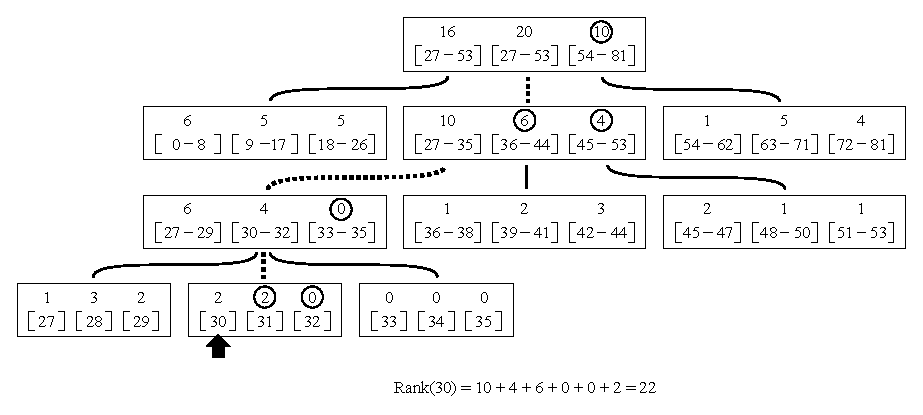
\includegraphics[width=15cm]{img/tree.eps}}
\end{figure}

\todo{Maybe do a better conclusion of pros and cons? Maybe a list?}

\section{Approximating algorithms}

Getting an exakt rank for a score may not be crucial. One fairly obvious class of solutions is the ones using linear interpolation of rank within a score range with known ranks at the boundaries. The ranks and score ranges needed for the interpolation may be acquired in different ways of which two will be described in this chapter; Buckets with Global Query and Frugal Streaming.

\subsection{How to measure error}

Approximating algorithms will almost by definition deviate from the \emph{true value} and we need a way to express that deviation.

One way could be expressing the error as the \emph{absolute error} as in. \ref{abs-error} \cite{pohl}.

\begin{equation}
  \label{abs-error}
  \varepsilon_{abs} = x_0 - x = \frac{\Delta x}{x} 
\end{equation}

$x$ is the true value and $x_0$ is in this case our approximated value. Another option would be expressing the error as the \emph{relative error} which is the quota between the absolute error and the true value \cite{pohl}.

\begin{equation}
  \label{rel-error}
  \varepsilon_{rel} = \frac{x_0 - x}{x} = \frac{\Delta x}{x} 
\end{equation}

A consequence of measuring the relative error when it comes to ranking is that a small rank estimate error will generate a large error when the estimating a high rank, and a relatively small error when estimating lower ranks with the same ranking error in absolute terms, for example see \ref{e1} and \ref{e2} where $|\Delta x| = 1$ in both cases.

\begin{equation}
  \label{e1}
x_0 = 9, x = 10 \quad \implies \quad \varepsilon_{rel} = \frac{9 - 10}{10} = -0.1  
\end{equation}

\begin{equation}
  \label{e2}
x_0 = 999, x = 1000 \quad \implies \quad \varepsilon_{rel} = \frac{999 - 1000}{1000} = -0.001  
  \end{equation}

Which way to go is of course application-dependent, but in the context of  ranking highscores in games the relative error is a very practical measure because it fits the real world concerns very well.

\subsection{\label{bucket}Buckets with Global Query}

The most basic way to go with the linear interpolation approach is called \emph{Bucket with Global Query} in the article \href{https://cloud.google.com/datastore/docs/articles/fast-and-reliable-ranking-in-datastore/}{Fast and Reliable Ranking in Datastore} \cite{ranking-in-datastore}. 

A background job periodically scans all highscores, creating a table with entries for scores and corresponding ranks. An excerpt from the created bucket-table may look like table \ref{table:ranking-table}. So, for example, to estimate the rank for score $2\;050$ which falls in bucket 6, start by calculating what the score range in bucket 6 is, in this case $2\;204 - 1\;961 = 243$. $2\;050$ is $89$ scorepoints ``in'' the bucket and hence the rank is calculated as $83 + 23 \times \frac{89}{243} \approx 91$. The same calculation is illustrated in figure \ref{fig:linear}.

\begin{figure}[h!]
  \centering
  \caption{Linear interpolation}
  \label{fig:linear}
  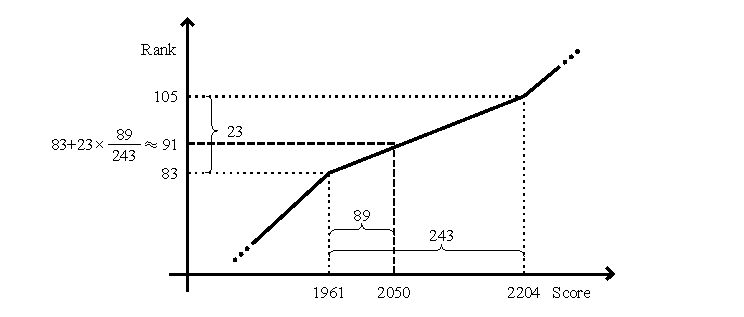
\includegraphics[width=13cm]{img/linear_interpolation.eps}
\end{figure}

\begin{table}[h]
  \begin{center}
  \begin{tabular}{ c c c c }
    Bucket no & Start score & Start rank & Size \\
    5 & 1 515 & 83 & 22 \\ 
    6 & 1 961 & 105 & 23 \\ 
    7 & 2 204 & 128 & 23 \\ 
    8 & 2 574 & 151 & 24 \\  
    9 & 2 852 & 175 & 25 \\ 
  \end{tabular} 
  \caption{Excerpt from bucket-table}
  \label{table:ranking-table}
  \end{center} 
\end{table}

The quality of the estimates made by this method depends on several factors.
\textbf{The frequency of the periodic scans} needs to be high enough to keep the error of the estimate at an acceptable level. Also, \textbf{the size of the buckets} have an impact on the result. Yet another factor that cannot be handled in a simple way is when the score \textbf{distribution within a bucket is skewed} or simply not very linear within the score range as in figure \ref{fig:uneven}.

\begin{figure}[h!]
  \centering
  \caption{An example of an uneven distribution of highscores within a bucket.
    In this case, a score in the middle of the actual distribution in the beginning of bucket a would get a rank estimate based on the score range defined by start scores of bucket a and b, which in this example would result in to a higher rank than the actual.}
  \label{fig:uneven}
  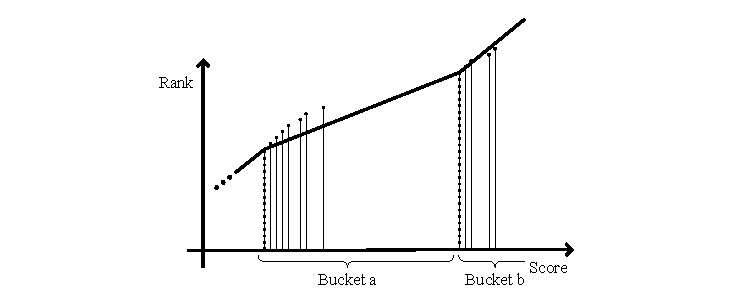
\includegraphics[width=13cm]{img/uneven_distribution.eps}
\end{figure}

If an update of a highscore from a lower score to a higher occurs but the new score is within the the same bucket as the previous score, the subsequent estimate will be the same for any score since the bucket-table is unchanged. Because the underlying distribution is changed the error may be different but not necessarily worse.

\todo{Illustration}

On the other hand, if a highscore estimate goes from a lower rank bucket to a higher one, a subsequent scan of the highscores would result in a table where the new bucket will grow by one and, start-rank of buckets after the new to and including the former one will increase by one and the bucket for the previous estimate would shrink by one.

\todo{Illustration}

% \begin{figure}[h]
%  \centering
%  \caption{A new highscore breaking the bucket-table}
%  \label{fig:change-buckets}
%  
\includegraphics[width=8cm]{img/change-buckets.png}
%\end{figure}

Future highscore updates will add to the bucket-tables deviation from a theorethical \emph{true} bucket-table and as a consequence the estimates will show a growing error with respect to the true rank until the bucket-table is recreated (Figure \ref{fig:errortime}). It is worth noting that the error should not be expected to be zero even with a fresh bucket-table since estimates is precisely that -- estimates.

\begin{figure}[h]
  \centering
  \caption{Error in estimates will grow over time, until the bucket-table is recreated and the error level drops down to the initial error. Bucket-table recreated at $t_0, t_1, t_2 \dots$. 
  }
  \label{fig:errortime}
  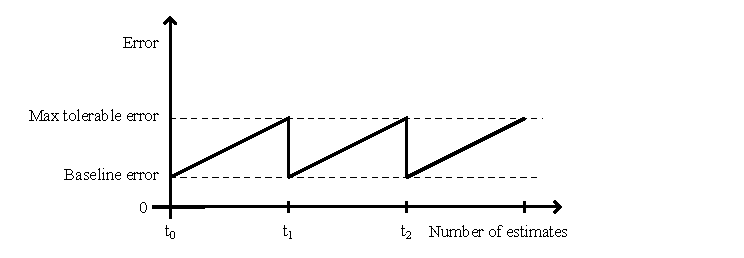
\includegraphics[width=13cm]{img/error-over-time.eps}
\end{figure}

\subsubsection{Handling errors caused by approximation}

A common requirement is that ranking have to be more precise, that is having a small $\varepsilon_{abs}$, for higher ranks than for lower ranks. This may be accomplished by having small buckets for higher ranks while increasing the bucket size by some formula for the lower ranks as in figure \ref{fig:growing}.  By using this method higher ranks will be predicted with better precision and the bucket-table will stay reasonably small. In some cases even an exponential bucket-growth will produce good enough result for the application.
 
\begin{figure}[h!]
  \centering
  \caption{Growing bucket sizes with critical section for which ranks are not estimated.}
  \label{fig:growing}
  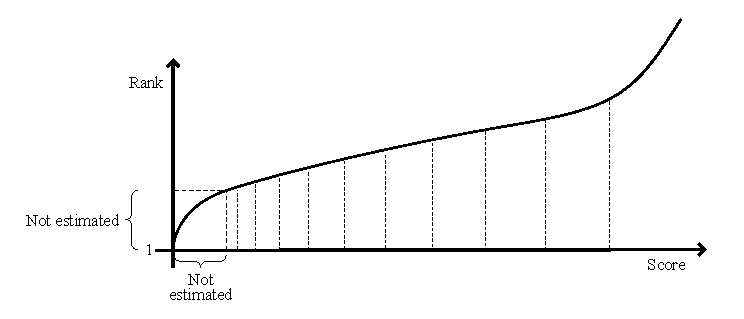
\includegraphics[width=13cm]{img/growing_bucket_sizes.eps}
\end{figure}

However, the method described above may not be enough to handle the highest ranks. One reason for that may simply be that the requirements on the algorithm and ultimately the final solution do not accept approximations \emph{at all} for the top ranks. To solve that problem this algorithm can be paired with the \emph{Rank by counting}-algorithm for the highest ranks. This should not be a problem since  the counting involves only the critical and highest ranks which can easily be fetched if the data is indexed. When to not estimate can be decided by looking at variables such as the score or rank estimate. 

\subsection{Online approaches, streaming algorithms}

\begin{mdframed}[backgroundcolor=red,innerleftmargin=15pt,leftmargin=-10pt,rightmargin=-10pt, innerrightmargin=15pt,innertopmargin=10pt,innerbottommargin=10pt, fontcolor=white, skipabove=20pt, linewidth=0]
  \textbf{The rest of the chapter is not really comprehendable in its current state. I intend to finnish this section later.}
  
\end{mdframed}

The drawback with the method described above is that the bucket-table after some time will no longer represent the actual distribution of scores and consequently less and less accurate rankings.

An alternative but still similar way of solving the problem could be by estimating a number of quantiles of the distribution of highscores by using a streaming algorithm. 

\emph{Frugal streaming} is a streaming streaming algorithm for estimating a quantile of a stream devised by Ma, Muthukrishnan and Sandler. \cite{frugal_streaming} The algorithm itself is fairly self explanatory (see appendix \ref{frugal}) and have a small memory footprint.

The idea is that by calculating a number of quantiles for every new highscore while keeping track of the total number of highscores you could create a bucket-table as in the algorithm described in section \ref{bucket}.

Calculating exact quantiles of a large dataset is quite expensive.

\subsection{Quantile Digest}

\emph{Quantile Digest} is a tree based stream summary algorithm. The paper that describes the algorithm does it from a sensor network perspective 
The algorithm builds a binary tree of the value domain. The tree is then compressed and can be sent to the parent of the sensor. The compression is lossy such that less frequent values are represented as a bucket. The result of the compression is called Quantile Digest.

Quantile query - inverse quantile

\blockquote{

Inverse Quantile: Given a value x, determine its
rank in the sorted sequence of the input values.
175
In this case, we again make the same sorted list (L),
and traverse it from beginning to end. We report the
sum of counts of buckets $v$ for which $x > v.max$ as
the rank of x. The reported rank is between rank(x)
and rank(x) + $\varepsilon$, $rank(x)$ being the actual rank of
$x$.}
